\documentclass{article}
\usepackage{graphicx} % برای اضافه کردن عکس
\usepackage{listings} % Load the listings package
\usepackage{xcolor}   % Optional: For custom colors
\usepackage{xepersian} % Persian support
\settextfont{XB Niloofar} % Change to a Persian font installed on your system

\lstset{
    language=C++,                      % Set language to C++
    basicstyle=\ttfamily\small,        % Use monospaced font
    keywordstyle=\bfseries\color{blue}, % Keywords in bold blue
    stringstyle=\color{red},           % Strings in red
    commentstyle=\itshape\color{green!60!black}, % Comments in green italics
    numbers=left,                      % Line numbers on the left
    numberstyle=\tiny,                 % Line number font size
    stepnumber=1,                      % Show line numbers every line
    frame=single,                      % Add a frame around code
    tabsize=4,                         % Set tab size
    showstringspaces=false             % Do not show spaces in strings
}

\begin{document}

\section*{تقدم عملگر‌ها}

در زبان C++ ترتیب و نحوه ارزیابی عملگر‌ها به دو مفهوم تقدم (Precedence) و وابستگی (Associativity) عملگر‌ها وابسته است. هر دو این مفاهیم مرتبط با زمان کامپایل کد هستند.

تقدم عملگرها مشخص می‌کند که در یک عبارت که شامل چندین عملگر است، کدام عملگر ابتدا اجرا شود و وابستگی عملگرها مشخص می‌کند که اگر چندین عملگر با تقدم یکسان در یک عبارت وجود داشته باشند، کدام یک ابتدا ارزیابی شوند.


\begin{figure}[h!]
    \centering
    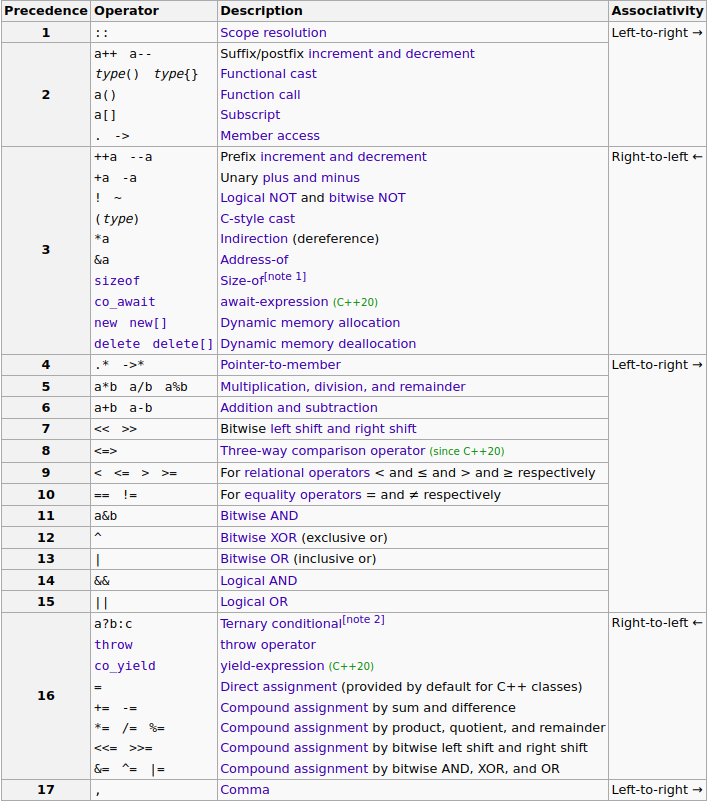
\includegraphics[width=0.7\textwidth]{1-operations.png}
    \caption{تمام عملگرهای زبان C++ به همراه تقدم و وابستگی}
    \label{fig:example}
\end{figure}


\end{document}
